\documentclass{standalone}
\usepackage{tikz}

\begin{document}

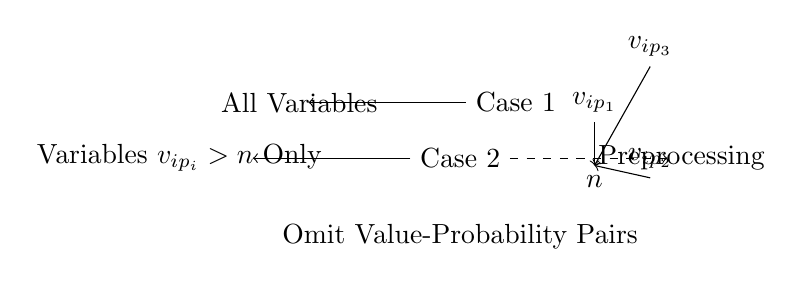
\begin{tikzpicture}[node distance=1cm]

    % Nodes representing the different cases
    \node (case1) {Case 1};
    \node (case2) [below left of=case1] {Case 2};
    
    % Nodes representing the variables and their values
    \node (var1) [right of=case1] {$v_{ip_1}$};
    \node (var2) [below right of=var1] {$v_{ip_2}$};
    \node (var3) [above right of=var1] {$v_{ip_3}$};
    
    % Nodes representing the threshold n
    \node (threshold) [below of=var1] {$n$};
    
    % Arrows showing the conditions for each case
    \draw[->] (case1.west) -- node[anchor=east]{All Variables} ++(-2,0);
    \draw[->] (case2.west) -- node[anchor=east]{Variables $v_{ip_i} > n$ Only} ++(-2,0);
    
    % Arrows showing the preprocessing step
    \draw[dashed,->] (case2.east) -- node[anchor=west]{Preprocessing} ++(2,0);
    \node (preprocess) [below of=case2] {Omit Value-Probability Pairs};
    
    % Connections between nodes
    \draw[->] (var1.south) -- (threshold.north);
    \draw[->] (var2.south) -- (threshold.north);
    \draw[->] (var3.south) -- (threshold.north);
    
\end{tikzpicture}

\end{document}